\documentclass{llncs}

\pdfoutput=1


\usepackage[cmex10]{amsmath}
\usepackage[pdftex]{graphicx}
\graphicspath{{./img/}}
\DeclareGraphicsExtensions{.pdf,.jpeg,.png}

\usepackage{rotating}
\usepackage{multirow}
\usepackage{url}
\usepackage{array}
\usepackage{subfigure}

\newtheorem{de}{Definition}

\hyphenation{co-ve-ra-ge}
\hyphenation{ge-ne-ra-ted}
\hyphenation{tool-chain}
\hyphenation{Sta-te-ma-chi-ne}

\begin{document}
\title{Applying a Def-Use approach on signal
exchange to implement SysML Model-Based Testing}

\author{Fabrice Ambert\inst{1} \and Fabrice Bouquet\inst{1} \and
  Jonathan Lasalle\inst{1} \and \\ Bruno Legeard\inst{1,2} \and
  Fabien Peureux\inst{1,2} }

\authorrunning{F.Ambert et al.}

\institute{FEMTO-ST Institute, UMR CNRS 6174, Besancon, France.\\
\email{\{fambert,fbouquet,jlasalle,blegeard,fpeureux\}@femto-st.fr},
\and
Smartesting R\&D Center, Besancon, France.\\
\email{\{legeard,peureux\}@smartesting.com}}

\maketitle

\begin{abstract}
Model-Based Testing (MBT) uses a model of the System Under Test as
reference to automatically derive test cases. Since it is often not
reasonable to cover all the behaviours formalized in the model,
coverage criteria are applied to select a relevant subset of model
behaviours. In this paper, we propose a dedicated test coverage
criterion, based on Def-Use criteria on signal exchange, to implement
MBT approach from \textit{Systems Modeling Language} (SysML) test
models to validate mechatronic systems. This novel criterion is
introduced and the relevance of the approach from SysML models is
discussed regarding results obtained with a dedicated MBT toolchain 
implementing this criterion. 
\keywords{Model-Based Testing, UML/SysML notations, coverage criteria, 
  mechatronic systems, toolchain experimentation}
\end{abstract}


\section{Introduction}
Model-Based Testing (MBT) refers to the processes and techniques
dealing with the automatic derivation of abstract test cases
(including stimuli and expected outputs) from an abstract formal
model, and the generation of executable tests from these abstract test 
cases~\cite{UL06}. MBT is usually performed to automate and
rationalize functional black-box testing activities. The
abstract model, called test model, formalizes the
behavioural aspects of the System Under Test (SUT) in the context of
its environment and at a given level of abstraction. It thus captures
the control and observation points, the expected dynamic behaviour,
the data associated with the tests, and finally the initial state of
the SUT. The test model must be precise and formal enough to enable
unambiguous interpretations to automate the derivation of test
cases.  
UML4MBT approach~\cite{bglp08} enables automated functional test generation
from a UML test model written with a subset of UML language~\cite{UML04} and OCL
constraints~\cite{OCL96}. These UML and OCL fragments are respectively
called UML4MBT and OCL4MBT~\cite{bglp07}. Basically, class diagrams
define the points of control and observation of the
SUT, instance diagrams define the initial state of the SUT
and give the set of the test data, while Statemachines with OCL
constraints define the expected behaviours in a formal way. 

\begin{figure}[htp]
	\centering
        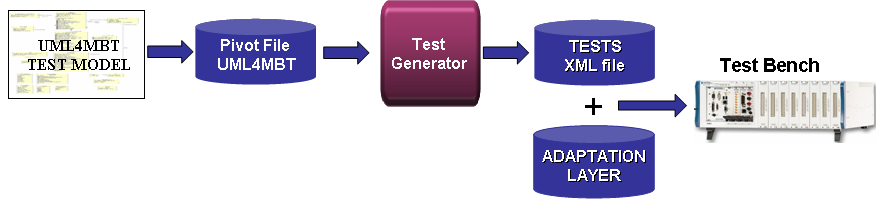
\includegraphics[width=10cm]{./img/initialToolChain.png}
	\caption{UML4MBT existing toolchain.}
	\label{UML4MBTToolChain}
        \vspace*{-.6cm}
\end{figure}

This MBT solution is implemented by the toolchain depicted in 
Fig.~\ref{UML4MBTToolChain}. It takes as input a test model specified by the
UML4MBT/OCL4MBT language, which has a precise and unambiguous 
meaning. OCL4MBT expressions indeed provide the expected level of
formalization necessary for model-based testing modeling. This precise
meaning makes it possible to simulate the execution of the models and
to automatically generate test cases. Such a test case
takes the form of an abstract sequence (abstract because it is
defined at the abstraction level of the test model) of the high-level
actions modeled in the test model. These generated test cases contain
the stimuli to be executed on the SUT, but also the expected results,
obtained by resolving the associated OCL constraints. Finally, the
test cases are concretized into executable scripts to be
automatically executed on the targeted testing platform.   

Since there is usually an infinite number of possible test cases that
can be generated from a test model, some test selection criteria have
to be applied to select a subset of appropriate test cases regarding
the global purpose of the test campaign, and/or to ensure a given
coverage of the system behaviours. Test selection criteria are usually
based either on control-flow coverage~\cite{OXL99} (such as
all-states, all-transitions, all-k-paths, etc.), or data-flow
coverage~\cite{RW85} (such as All-Defs, All-Uses, All-DU-Paths,
etc.). Moreover, condition coverage criteria~\cite{Vilkomir01} (such as
CC, DC, D/CC, MC/DC, etc.) may additionally be applied to enforce the
structural coverage of the decisions of the test model. The test
coverage strategy applied by the UML4MBT approach relies both on
control-flow and condition coverage criteria: UML4MBT applies
$All~transitions$ coverage, which ensures to cover each
transition of the UML4MBT Statemachines, and Decision/Condition
Coverage (D/CC) criterion, which ensures the coverage of all the
conditions and all the decisions of the UML4OCL annotations. 

In this paper, we propose to extend the UML4MBT solution to
specifically address embedded mechatronic system domain. We thus
propose to adapt this existing approach by taking \textit{Systems
  Modeling Language}~\cite{FMS09}~(SysML) as input test models, and 
by introducing a dedicated coverage criterion, called
\texttt{ComCover}, to select relevant test cases from such models. 
A fully automated toolchain, supporting this MBT process, is also 
introduced and experimentation results are provided. 
The paper is organized as follows. Section~\ref{relatedWorks}
introduces the motivation and the context of this
research. Section~\ref{modeling} defines the subset of SysML notation
supported to express the test model. Section~\ref{comCover}
and~\ref{formalization} respectively describe and formalize the
original \texttt{ComCover} criterion dedicated to such test
models. Section~\ref{tool} briefly presents the toolchain supporting
this approach and discusses case study
results. Section~\ref{conclusion} finally concludes the paper. 

\section{Related Works}
\label{relatedWorks}
Mechatronic systems refer to systems that combine software,
electronical systems and additional mechanical parts to perform a 
dedicated function. In this context, embedded softwares define a part
of a larger system or product. Then, we can deduce that the embedded
system exists because the larger system needs it. That is why testing
an embedded system, without considering the system containing it, is
often not efficient. In order to completely analyze and validate this
kind of system, it appears necessary to take into account all
parts which influences it. 

Since 1990, the well-know simulation program PELOPS\footnote{See
  \url{http://www.pelops.de/UK/index.html}} is developed on the idea
that, to specify a vehicle embedded systems in order to analyze it, it
is necessary to represent three specific parts: the vehicle, the
driver and the environment~\cite{EHMANNS2000}.
This realistic kind of modeling can then be validated by simulation:
theoretical results calculated using such model framework are indeed
compared with concrete results given by the physical corresponding
system~\cite{GLASER2002}. These three parts have to contain all
elements that can influence the behaviour of the embedded system. This 
framework is nowadays still used in several works, and defines the
preamble of the work presented in this paper. However, taking into
account each environment part usually introduces combinatorial
explosion problems, especially when each system part is tested
independently. Moreover, in order to detect undesired
behaviour, it is necessary to study interaction network between all
the system components~\cite{Petin}. Consequently, our approach does
not consist in verifying properties by proving local properties of
each component, but in considering the global system components by
focusing on their interactions. 

A major challenge of such approaches concerns the heterogeneity of
the different components and technology domains. To address this issue,
it is needed to make uniform the representation of components at a
given and adequate abstract level. \cite{Bonfe}~shows that using UML/SysML based
models is an efficient way for automation engineering to handle the complexity
of embedded systems. In this way, to avoid combinatorial problems, it
is necessary to capture in the context model only the information
required to simulate the behaviour of the system with regards to the
evolution of its environment. 

Several testing approaches for embedded systems are based on a model
of the SUT environment. Typically, as
proposed in~\cite{Simula}, a test case is defined as a sequence of
stimuli that are sent from the environment to the embedded system
under test. In order to
generate test cases, the authors apply Adaptive Random Testing
and Search-Based Testing. These techniques allow to reduce
combinatorial explosion during calculation, but gives poor information
about the coverage of the test model and make difficult to assess a
certain coverage.

Concerning the choice of the modelling language, two main strategies
have been explored. As shown in~\cite{Thacker}, the first approach
promotes the use of formal and mathematical languages such as Petri
nets and VHDL-AMS codes. This kind of languages is powerful to
specify mathematical and physical expressions, but they are not easy
to acquire and does not often correspond to software engineer
knowledge. Indeed, to be admitted by the software engineers, such
approaches need to use a language widely used by software
engineers. This point of view notably motivates the second approach
that considers less formal, and often graphical, models. Moreover, in
practice, starting the analysis of complex system using too concrete
models is not convenient: it is usually necessary to begin the study
using a more abstract notation in order to master the complexity of
such systems. In this way, in~\cite{SimulaEnvModeling}, the authors
propose to develop a domain model with UML class Diagram to represent
the global structure of the environment (relationships, properties and
constraints). Several behavioral models for each environment parts are
also designed using UML Statemachines to model the dynamic part of the
system. Other UML-based approaches use sequence diagrams,
as~\cite{Testbenches}, to model behavioural aspects or to represent
test classification trees. In~\cite{Evrot}, the authors propose to use
SysML to initially specify the system in a graphical manner. This
language, where the object-oriented features are not visible, makes it
possible to capture the mechatronic aspects of the SUT, and ease the
interaction between different teams of multi-domain engineers.

In this paper, we also propose to use the Unified Modeling Language
paradigm. This notation gives the advantage to be widely supported in
terms of tools and training material. More precisely, we adopt SysML as
specification language. Even if SysML is a recent modeling language,
it is indeed on the rise in embedded system domain and some studies
already use it to develop new industrial validation approaches
(e.g. Model Checking and testing of on-board space
applications~\cite{FMS99}). Moreover, SysML, being defined as an OMG 
standard profile of UML, makes it possible to reuse
existing testing approaches and tooling based on UML test models. In
this way, it allows to adapt the existing UML4MBT approaches by
focusing on the specific needs of testing mechatronic systems.  

\section{SysML4MBT Modeling}
\label{modeling}
This section describes the subset of SysML notation supported to
express the test model. This description is based on a simplified
version of a realistic case study that will be used in the next
sections to illustrate our approach.

\subsection{Emergency-Stop Case Study}
The emergency-stop case study describes a train emergency-stop
system. This example will be used in the next sections to illustrate
the proposed MBT approach. This system is defined by the following
functionalities and rules: 
\begin{itemize}
\vspace*{-.25cm}
  \item The train can either be stationing or moving on rail track.
  \item It is possible to set off the $emergency-stop$ by pulling the button
  $button1$.
  \item It is possible to set off the $emergency-stop$ by
    pushing the button $button2$. 
  \item When one of these two buttons is activated, a signal is sent to the
  emergency-stop manager system, which automatically stops the train
  and sets off the alarm if the train is moving, or only advises the
  driver if the train is stopped. 
\end{itemize}

To model this system, it is necessary to represent mechanical parts
(buttons for example) and communications between subsystems (buttons
and emergency-stop manager system) using signal. Mechatronic systems
are indeed typically composed of some logical and some physical parts 
that communicate using mechanical or physical signals. But UML4MBT is not 
adapted to cover such aspects: a UML4MBT class
diagram represents a logical entity of the system, and not at
all a physical system; classes contain operations and attributes but
signals are not allowed; only one Statemachine annotated by OCL
expressions is allowed; neither parallel structures (parallel states,
fork and join states) nor historic states are supported in the
Statemachine; etc. 
That is why we decided to extend the expressiveness of UML4MBT to model 
parallel Statemachines and structures, and communication network between the subsystems of the SUT by taking 
into account the communication ports and links. Moreover, we also decided 
to use a subset of the SysML profile notation to capture the semantics of such
embedded systems. It
should be noted that the representation of time constraints, which
is an other major aspect of embedded systems, will
not be considered in the current approach, but will be studied in
future work by using a dedicated UML extension such as
MARTE profile~\cite{Marte}.
\vspace*{-.25cm}
\subsection{SysML4MBT Expressiveness}

The test model, specified by SysML diagrams, defines the expected
behavior of the SUT: it formalizes the control and observation points 
of the SUT, and its expected behaviour. However, SysML contains a
large set of diagrams that defines a flexible notation and presents 
some freedom that can offer different semantical
interpretations. For practical MBT, it is necessary to select a
subset of SysML, and to clarify its semantics so that MBT tools can
interpret the models in a unambiguous way. We thus define a precise
subset of SysML for test generation purpose called SysML4MBT. A 
SysML4MBT model is composed of the following entities:  
\begin{itemize}
\vspace*{-.25cm}
  \item A Block Definition Diagram (BDD) represents the static view of the
  system. It is defined as a stereotype of the UML class
  diagram. It can contain blocks, associations, compositions, signals,
  flow specifications and enumerations. 
  \item An Internal Block Diagram (IBD) represents the internal view of the
  system, providing interconnections between its physical parts. The SysML IBD is
  defined as a stereotype of the UML Composite Structure Diagram.
  \item One or more Statemachines specify the dynamical view of the
    system. SysML Statemachines are directly inherited from UML
    Statemachines. Additionally to UML4MBT, SysML4MBT enables parallel
    structures (parallel states, fork/join states and multiple
    Statemachines) and historic states. 
  \item In order to represent in a formal way the dynamical aspect of
    the system, OCL4MBT constraints are used to define the pre and
    post-conditions of the operations, and the guards and effects of
    the transitions in the Statemachine. The circumflex operator,
    which represents a sent signal in OCL, has been added to the
    OCL4MBT initial expressiveness.  
\end{itemize}
\vspace*{-.4cm}
\subsection{SysML4MBT Modeling}
\vspace*{-.1cm}
To model the emergency-stop system, the train can be divided into
three parts: the first part defines the general state of the train,
the second one defines the button system, and the third one specifies
the emergency-stop manager. It should be noted that, due to their
simplicity and to simplify the presentation, only Statemachines are 
presented and depicted in Fig.~\ref{trainStatemachine} (BDD and IBD
are not shown in this paper), and actions are all abstracted in the
Statemachines. Finally, each transition is identified by a label {\tt
  trX} to ease the explanation understanding.
\vspace*{-.5cm}
\begin{figure}[htp]
\center{
  \subfigure[Train]{\fbox{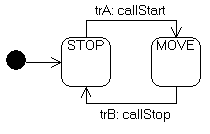
\includegraphics[width=3.9cm]{./img/example/general.png}}}
\quad
  \subfigure[Button]{\fbox{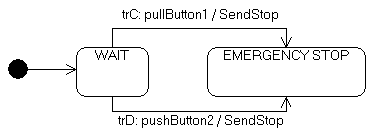
\includegraphics[width=7cm]{./img/example/buttons.png}}
	\label{emergencyButtons}}}\\
\centerline{
  \subfigure[Emergency]{\fbox{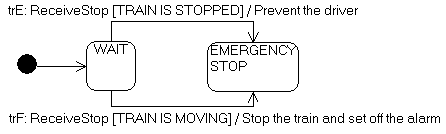
\includegraphics[width=8cm]{./img/example/management.png}}
	\label{emergencyManagement}}\vspace{-.3cm}}
\caption{Statemachines of the emergency-stop case study}
\label{trainStatemachine}
\end{figure}
\vspace{-.5cm}

The Statemachine defining the behaviour of the train, contains two
states: $STOP$ (the train is stationing) and $MOVE$ (the train is
moving). The expression $callStart$ (resp. $callStop$) represents a
call of $start$ (resp. $stop$) operation that is a request to move
(resp. stop) the train.  
At the initial state, the button system is waiting for an activation
of one of the buttons. When one of them is activated (action
$pullButton1$ if the button1 is pulled, and action $pushButton2$ if
the button2 is pushed), a signal is sent to the emergency manager
system. The sending of this signal is modeled by the action $SendStop$.
Finally, the emergency-stop manager is initially positioned in the
state $WAIT$. When it receives the emergency-stop signal sent by the
button system (transition triggered by $ReceiveStop$), the train will
stop and the alarm will be set off if the train is moving (guard of
the transition); else, it only prevents the driver. 
This example will be used in the rest of the paper to
illustrate the SysML4MBT testing approach. 

\vspace*{-.25cm}
\section{Test Model Coverage Strategies}
\label{comCover}
\vspace*{-.25cm}
Some well-known criteria are usually used in Model-Based Testing
techniques. A hierarchy of structural coverage criteria is notably defined
in~\cite{FW88} as depicted in Fig.~\ref{initialCriteria}.  
Criteria in the box are control-flow criteria and the others are data-flow 
criteria, while the (inheritance) arrows define that if the criterion at the 
start of the arrow is covered, the criterion pointed by this arrow is also 
covered.

The criterion $All~states$ consists in the coverage of each state of
the model, while $All~transitions$ ensures that each transition is
covered. It means that for each state (resp. transition), at least one
test case executes it (if it is feasible). The criterion $All~DU$
(shortcut for {\it All~Definition/Use}) deals with the coverage of
each couple of definition (update) and use (reading) of each
variable. It means that each time a variable is modified in the model,
for each time it is read, a test, executing the definition before
executing the use of the variable (without executing an other
definition meantime) has to be generated. The criterion $All~DU$ is
defined as an extension of the $All~transitions$ criterion: it ensures
the coverage of all transitions and all definition/use pairs. The
criterion $All~DU-paths$ suggests the same level of coverage as
$All~DU$, but apply the approach to cover, for each variable, all the
possible paths linking a definition and a use. Finally, the most
constrained criterion of this hierarchy is the criterion $All~paths$:
it guarantees the coverage of all the possible paths in the
system. The $All~DU-paths$ and $All~paths$ criteria are infeasible in
practice due to combinatorial explosion of reachable states, and can
be usually applied only on very small models since it generates a
large number (potentially infinite) of test cases. 

\subsection{Strategy implemented within UML4MBT}

The test coverage strategy implemented within UML4MBT relies on
control-flow and condition coverage criteria. UML4MBT applies
$All~transitions$ that ensures to cover each transition, and also
implements  Decision/Condition Coverage criterion (D/CC) for each
decision branch of the model. The D/CC criterion deals with the
coverage of all the conditions and all the decision of the model. It
means that for each effect of each transition, the condition of
decision structure and the decision itself have to be true and false
in at least one test case.

These criteria do not take into account particularities of SysML
models. Indeed, a major issue of SysML4MBT models in
comparison with UML4MBT models concern the representation of
communication links and exchanges (send and receive of signals)
between components of the system. The next subsection underlines this
lack of the UML4MBT approach on the emergency-stop example.
\vspace*{-.4cm}

\subsection{Illustration of the UML4MBT Strategy}

The three Statemachines of the case study model contain six
transitions. Each one contains only one behaviour without
condition. Then, the application of the $All~Transitions$ criterion is 
sufficient and the D/CC criterion is of no interest in this case. 
By performing UML4MBT approach to this model, the test cases represented 
in Table~\ref{genUML4MBT-jouet} are generated (in the representation of
test cases, elements in parenthesis represent automatically fired
transitions, while elements into brackets gives the name of the
corresponding transition).

\begin{table}[htp]
\centering
\vspace*{-.4cm}
\caption{Tests generated using UML4MBT strategy.}
\begin{small}
\begin{tabular}{|m{3.4cm}|c| m{3.2cm}|}
	\hline
	\multicolumn{1}{|c}{Targets} & \multicolumn{1}{|c|}{Id} & \multicolumn{1}{|c|}{Tests}
	\\ \hline
	\multicolumn{3}{|c|}{Train state Statemachine}
	\\ \hline
	trA \newline Start the train.
	&S1& $callStart[trA]$ 
	\\ \hline
	trB \newline Stop the train.
	&S2&  $callStart[trA]$\newline
	$\rightarrow callStop [trB]$
	\\ \hline
	\multicolumn{3}{|c|}{Button system Statemachine}
	\\ \hline
	trC \newline Pull the button 1. 
	&S3& $pullButton1 [trC]$\newline
	$\rightarrow (ReceiveStop[trE])$
	\\ \hline
	trD \newline Push the button 2.
	&S4& $pushButton2 [trD]$\newline
	$\rightarrow (ReceiveStop[trE])$
	\\ \hline
	\multicolumn{3}{|c|}{Emergency manager Statemachine}
	\\ \hline
	trE \newline Emergency stop called \newline (train already stopped).
	& & Already covered by S3 and S4.
	\\ \hline
	trF \newline Emergency stop called \newline (train moving).
	&S5& 
	$callStart [trA]$\newline
	$\rightarrow pullButton1[trC]$\newline
	$\rightarrow (ReceiveStop[trF])$
	\\ \hline
\end{tabular}
\end{small}
\label{genUML4MBT-jouet}
\vspace*{-.4cm}
\end{table}

Since the sequence S1 is included in S2, S1 is not required. Thus,
to satisfy the coverage criterion $All~Transitions$, the four test cases
represented by the sequences S2, S3, S4 and S5 are generated by the
UML4MBT approach.

This example shows that there is a deficiency on the case study coverage
because the scenario, consisting to push the button2 when the train is
moving, is not required to satisfy the criterion. In critical system
context, it appears to be necessary to test such case. Then, to avoid
this lack, a more precise strategy should be applied: for this
purpose, a dedicated data-flow test selection strategy, called
\texttt{ComCover}, has been defined to cover all the configurations of signal
exchange. The next subsection introduces this dedicated criterion and
defines it with regards to the previously presented criteria.
\vspace*{-.4cm}

\subsection{ComCover Strategy}

Within SysML4MBT test generation strategy, we are interested in the
coverage of each signal received from each signal sending. In this way,
we propose to adapt the $DU$ approach, which concerns variables of the
system, to address the exchange of signals in order to create a
sensible test metric for reactive parallel Statemachines. This
original criterion is called $All~DU_{sig}$, and the corresponding
strategy to select test cases, that satisfy this criterion, is called
\texttt{ComCover}. 

The $All~DU_{sig}$ criterion, based on $All~DU$, deals with the coverage of
send and receive events. The criterion $All~DU_{sig}$ guarantees the coverage of the
succession of the sending event and the receive event: For each
transition pair that is synchronized on the same event (one sender and
one receiver), a test is required to show that the sender triggers the
receiver. In analogy with the
$All~DU$ criterion, the $All~DU_{sig}$ criterion can be seen as an extension
of the $All~transitions$ criterion. Thus, the $All~DU_{sig}$ criterion
ensures the coverage of all transitions and all send/receive
couples. Finally, we also define the 
$All~DU_{sig}-paths$ criterion, which guarantees, for each
send/receive couple, the coverage of all possible paths containing
them. The criteria hierarchy is updated as shown in
Fig.~\ref{newCriteria}. 

\begin{figure}[htp]
	\centering
\vspace*{-.4cm}
  \subfigure[Traditional hierarchy]{\fbox{\hspace*{.5cm}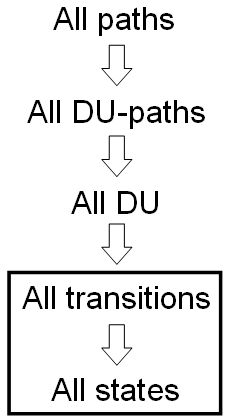
\includegraphics[width=2.27cm]{./img/oldhierarchie.png}\hspace*{.5cm}}
	\label{initialCriteria}}
\quad \quad \quad \quad
  \subfigure[Updated hierarchy]{\fbox{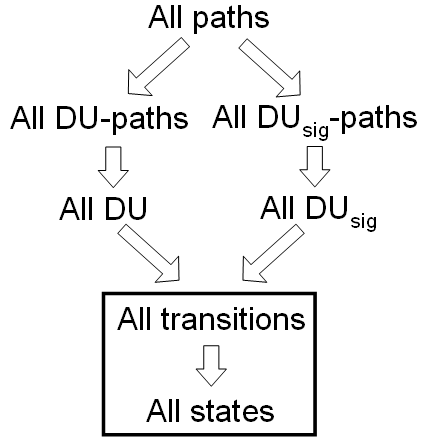
\includegraphics[width=4cm]{./img/newhierarchie.png}}}
\vspace*{-.2cm}
\caption{Hierarchy of test coverage criteria.}
\label{newCriteria}
\vspace*{-.4cm}
\end{figure}


The strategy, which consists in generating test cases in order to
guarantee the $All~DU_{sig}$ criterion, is called \texttt{ComCover}. The use of $All~DU_{sig}-paths$ as selection criterion has
not been implemented, and not be experimented, due to scalability 
issues. Indeed, $All~DU-paths$ criteria is known to be infeasible in
practice since it results in an infinite number of tests when
the Statemachine contains loops~\cite{weiss10}.   

The \texttt{ComCover} strategy is thus based on communications
between parts: its purpose is to extract all send/receive couples of
SysML4MBT Statemachines and to cover them by at least one test case
that fires the concerned signal receiving behaviour after having fired
its sending. Concretely, each behaviour $BhvA$ (of a transition in a
Statemachine) that sends a signal to a specific port, and each
behaviour $BhvB$ that can receive the signal sent by $BhvA$, are
extracted from the model. Each couple $BhvA$/$BhvB$ then constitutes a
test target to be covered by at least one test case to ensure $All~DU_{sig}$. 
\vspace*{-.25cm}
\subsection{Illustration of the ComCover Strategy}
\vspace*{-.25cm}
This section presents the results of the \texttt{ComCover} strategy
using the SysML4MBT emergency-stop example. This model contains two
signal sendings: $SendStop$ on the transition $trC$ and $SendStop$ on
$trD$. The receive of the signal can activate two transitions: $trE$
and $trF$. Then, four test targets can be derived: the couples C1 (by
firing $trC$ before $trE$), C2 (by firing $trC$ before $trF$), C3 (by
firing $trD$ before $trE$)and C4 (by firing $trD$ before $trF$).
The test cases of Table~\ref{genSysML4MBT-jouet} are then generated
using a classical breadth-search algorithm to cover each
couple. 

\begin{table}[htp]
\centering
\vspace*{-.25cm}
\caption{Test cases generated using ComCover.}

\begin{tabular}{|m{3.4cm}|c| m{3.2cm}|}
	\hline
	\multicolumn{1}{|c}{Targets} & \multicolumn{1}{|c|}{Id} & \multicolumn{1}{|c|}{Tests}
	\\ \hline
	C1 (trC/trE) \newline Pull the button 1 \newline (train already stopped).
	&S6& $pullButton1 [trC]$\newline
	$\rightarrow (ReceiveStop [trE])$
	\\ \hline
	C2 (trC/trF) \newline Pull the button 1 \newline (train moving).
	&S7& $callStart [trA]$\newline
	$\rightarrow pullButton1 [trC]$\newline
	$\rightarrow (ReceiveStop [trF])$
	\\ \hline
	C3 (trD/trE) \newline Push the button 2 \newline (train already stopped).
	&S8& $pushButton2 [trD]$\newline
	$\rightarrow (ReceiveStop [trE])$
	\\ \hline
	C4 (trD/trF) \newline Push the button 2 \newline (train moving).
	&S9& $callStart [trA]$\newline
	$\rightarrow pushButton2 [trD]$\newline
	$\rightarrow (ReceiveStop [trF])$
	\\ \hline
	\multicolumn{3}{|c|}{Complement to guarantee $All~transitions$}
	\\ \hline
	trB \newline Stop the train.
	&S10&$callStart[trA]$\newline
	$\rightarrow callStop [trB]$
	\\ \hline
\end{tabular}
\vspace*{-.35cm}
\label{genSysML4MBT-jouet}
\end{table}

In comparison with the results obtained using UML4MBT approach, S6 and S3 are
equals, like S8 and S4, S7 and S5, and S2 and S10. 
On this simple example, all
tests generated by the strategy of the UML4MBT approach are also generated with
the \texttt{ComCover} strategy.
Besides, the sequence that was missing using
UML4MBT approach (activation of the emergency-stop using the
button2 when the train is moving), is generated by \texttt{ComCover}
with the sequence S9.
\vspace*{-.25cm}
\section{Formalization}
\label{formalization}\vspace*{-.25cm}
This section introduces the formalization of the criteria $D/CC$
and $All~DU_{sig}$ on the basis of SysML4MBT
expressiveness. 
\vspace*{-.25cm}
\subsection{Formalization of a SysML4MBT Model}
\vspace*{-.25cm}
In this subsection, we introduce the subset of SysML4MBT
notation that is required to formalize the coverage criteria. All
elements annotated with~$*$ are not detailed here, but can be found 
in~\cite{UMLFM10}, where the SysML4MBT modeling notation is
completely formalized. 
A SysML4MBT model is composed of a Block Definition Diagram (BDD),
Internal Block Diagram (IBD) and one or more Statemachines
(SM). Internal Block Diagram, not required to formalize criteria, will
be ignored in the rest of this section. We adopt the same restrictions
for BDD in which only blocks and signals are relevant to define the
criteria.

 \begin{de}[Model]
A SysML4MBT model can be defined by the 2-tuple $\langle BDD,SMS
\rangle$, where $BDD$ represents the Block Definition Diagram and $SMS$
is a set of Statemachine Diagrams ($SM$). 
\end{de}

\begin{de}[BDD]
A BDD is defined by the 2-tuple $\langle SIGS,BLOCKS \rangle$,
where $SIGS$ is the set of all signals and $BLOCKS$ is the set
of all blocks. 
\end{de}

\begin{de}[Block]
A Block $BLOCK$ is defined by the 3-tuple $\langle OPS^*,$ \linebreak
$PROPS^*, PORTS^*\rangle$, where $OPS$ is a set of all operations,
$PROPS$ the set of all properties, and $PORTS$ the set of all ports
contained in the block.
\end{de}

To directly access to block elements of a model M, we
define the accessors $M.allProps$, $M.allOps$ and $M.allPorts$ that
respectively represent the set of all properties, operations and
ports of the model $M$. We can now formalize the SysML4MBT
Statemachine and its transitions. 
A transition starts from a state and reaches an other (which can be the
same), and can be guarded and triggered by an event. When this event
appends, if the guard of the transition holds, the transition is
fired and one of its behaviours is executed. 

\begin{de}[SM]
A Statemachine is represented by a 2-tuple $\langle STATES^*,$
\linebreak $TRANS \rangle$, where $STATES$ denotes all states of the
Statemachine Diagram, and $TRANS$ is a set of all transitions of the
Statemachine Diagram. 
\end{de}

\begin{de}[Transition]
A transition is defined by $\langle TRstart^*,TRend^*,$ \linebreak $TRtrig,TRguard^*,TRbhvs \rangle$
where:\vspace*{-.25cm}
\begin{itemize}
  \item $TRstart$ is the initial state of the transition.
  \item $TRend$ is the final state of the transition.
  \item $TRtrig$ corresponds to the trigger of the transition \\
  $TRtrig \in ((BDD.SIGS~*~allPorts)~\cup~allOps)$.
  \item $TRguard$ defines the guard of the transition.
  \item $TRbhvs$ contains all behaviours of the transition. 
\end{itemize}
\end{de}

The behaviours of the transition are defined by an effect and
a guard, which is a boolean expression on states that must hold to
execute the action. It is formalized in the following way. 

\begin{de}[Behaviour]
A behaviour is defined by a 2-tuple $\langle BHVdecision^*,$ \linebreak $
BHVaction \rangle$, where:\vspace*{-.25cm}
\begin{itemize}
  \item $BHVdecision$ defines the guard. 
  \item $BHVaction$ is the set of all effects that can be executed
    when the behaviour is activated. An effect takes the form of a
    signal sending on a specific port or an update of a property value:\\
  $(BDD.SIGS~*~allPorts)~\cup~(allProps~*~newValue)$ \\
  ($newValue$ represents the new value to be associated to the property). 
\end{itemize}
\end{de}

\subsection{Formalization of a Test Case}
\vspace*{-.25cm}
Within test generation from SysML4MBT models, we define a test
case as a trace (sequence) of steps (operation calls).
\vspace*{-.25cm}
\begin{de}[Trace]
$TRACES$ defines the set of all possible traces of the SysML4MBT
  model. A trace $tr$, such that $tr \in TRACES$, contains an ordered
  set of steps $\langle StepOP^*,StepBhv^*,AllBhvs^*
  \rangle$, where:\vspace*{-.25cm}
\begin{itemize}
  \item $StepOP$ defines the operation triggering the behaviour.
  \item $StepBhv$ is the executed behaviour if the trigger holds. 
  \item $AllBhvs$ is an ordered set containing all the behaviours
    (including $StepBhv$) triggered by $StepOP$.
\end{itemize}
\end{de}
\vspace{-0.3cm}
The set of generated test cases $TESTS$ is thus a subset of
$TRACES$ that contains all the traces selected by the test generation
strategy: $TESTS \subseteq TRACES$. All the elements, needed to
formalize the coverage criteria $D/CC$ and $All~DU_{sig}$ have
been introduced. 
\vspace*{-.3cm}
\subsection{Formalization of the Criteria}
\vspace*{-.25cm}
Using the definitions introduced in the previous subsection, we
firstly propose in Fig.~\ref{formaltrans}, the formalization of the 
criterion $all~transitions$ applied on UML4MBT model, which is refined
using SysML4MBT model by $All~DU_{sig}$ criterion.

\begin{figure}[htp]
\begin{center}
\begin{scriptsize}
\fbox{\begin{minipage}{\columnwidth}{
\begin{tabbing}
$\forall~trans.(trans \in \{t|\exists~sm.(sm \in M.SMS~\wedge$\\
~~~~~~~~~~~~~~~~~~~~~~~~~~~~~~~~~$t \in sm.TRANS)\}\Rightarrow$\\
~~~~$\exists~bhvTest.(bhvTest \in \{b|\exists~(step,t).(t \in TESTS~\wedge~step \in t~\wedge $\\
~~~~~~~~~~~~~~~~~~~~~~~~~~~~~~~~~$b \in step.AllBhvs)\}~\wedge$\\
~~~~~~~~~~~~~~~~~~~$bhvTest \in trans.TRbhvs))$
\end{tabbing}
}\end{minipage}}
\end{scriptsize}
\vspace*{-.2cm}
\caption{Formalization of $All~transitions$ criterion.}
\label{formaltrans}
\end{center}
\vspace*{-.8cm}
\end{figure}
The $All~DU_{sig}$ criterion, applied to SysML4MBT model to improve its coverage
regarding communication exchange, is defined in Fig.~\ref{formalALLDUsig}
(in this formalization, the formula $bhvSend~<_{step.AllBhvs}~bhvRec$
means that $bhvSend$ is before $bhvRec$ in the $step.AllBhvs$ ordered
set). Informally, this formalization establishes that a test set satisfies
this criterion if all pairs signal send/receive are covered by at least
one test case. The criterion $All~DU_{sig}-paths$ enforces this
criterion by ensuring the coverage of all paths that can be
used to provide the $All~DU_{sig}$ criterion (this criterion has not
been experimented due to scalability issues and is thus not formalized
in this paper).

\begin{figure}[htp]
\vspace*{-.25cm}
\begin{center}
\begin{scriptsize}
\fbox{\begin{minipage}{\columnwidth}{
\begin{tabbing}
$\forall~(sig,port,bhvSend,trRec).$\\
~~~~$((sig \in M.BDD.SIGS~\wedge~port \in M.allPorts()~\wedge$\\
~~~~$bhvSend \in \{b|\exists~(sm,t).(sm \in M.SMS~\wedge$\\
~~~~~~~~~~~~~~~~~~~~$t \in sm.TRANS~\wedge~b \in t.TRbhvs)\}~\wedge$\\
~~~~$trRec \in \{t|\exists~sm.(sm \in M.SMS~\wedge$\\
~~~~~~~~~~~~~~~~~~~~$t \in sm.TRANS)\}~\wedge$\\
~~~~$\langle sig,port \rangle \in bhvSend.BHVaction~\wedge$\\
~~~~$trRec.TRtrig~=~\langle sig,port \rangle)$\\
~~~~$\Rightarrow$ 
%~~~~
$\exists~(step,bhvRec).$\\
~~~~~~~~~~~~~~$(step \in \{s|\exists~t.(t \in TESTS~\wedge~s \in
t)\}~\wedge $\\
~~~~~~~~~~~~~~$bhvSend \in step.AllBhvs~\wedge $\\
~~~~~~~~~~~~~~$bhvRec \in step.AllBhvs~\wedge $\\
~~~~~~~~~~~~~~$bhvRec \in trRec.TRbhvs~\wedge $\\
~~~~~~~~~~~~~~$bhvSend~<_{step.AllBhvs}~bhvRec))$
\end{tabbing}
}\end{minipage}}
\end{scriptsize}
\vspace*{-.2cm}
\caption{Formalization of $All~DU_{sig}$ criterion.}
\label{formalALLDUsig}
\end{center}
\vspace*{-.8cm}
\end{figure}

Finally, we can use the formalization of a SysML4MBT model to
formalize the D/CC criterion, which is applied in our approach to
complete the previous data-flow strategies. This formalization is
expressed in Fig.~\ref{formalDCC}.

\begin{figure}[htp]
\vspace*{-.25cm}
\begin{center}
\begin{scriptsize}
\fbox{\begin{minipage}{\columnwidth}{
\begin{tabbing}
$\forall~bhv.(bhv \in \{b|\exists~(sm,t).(sm \in M.SMS~\wedge $\\
~~~~~~~~~~~~~~~~~~~~~~~~$t \in sm.TRANS~\wedge $
$b \in t.TRbhvs)\}$\\
~~~~$\Rightarrow \exists~bhvTest.(bhvTest \in \{b|\exists~(step,t).(t \in TESTS~\wedge $\\
~~~~~~~~~~~~~~~~~~~~~~~~~~~~~~~~~~~$step \in t~\wedge $
%~~~~~~~~~~~~~~~~~~~~~~~~~~~~
$b \in step.AllBhvs)\}~\wedge~bhvTest=bhv))$
\end{tabbing}
}\end{minipage}}
\end{scriptsize}
\vspace*{-.2cm}
\caption{Formalization of D/CC criterion.}
\label{formalDCC}
\end{center}
\vspace*{-1.2cm}
\end{figure}

\section{Toolchain and Experimentation Results}
\label{tool}
\vspace*{-.25cm}
The \texttt{ComCover} approach consists to automatically derive, from a
SysML4MBT model, test cases that satisfy $All~DU_{sig}$. Moreover, we
decide to ensure the D/CC criterion to cover the conditional branches
specified in the model. The toolchain implementing this approach from
SysML4MBT models is an extension of the existing UML4MBT toolchain
(Fig.~\ref{UML4MBTToolChain} in the introduction of this paper),
which derives test cases from UML4MBT model by computing both
$All~transitions$ and D/CC test selection strategies. 

The obtained
toolchain, depicted in Fig.~\ref{newToolChain}, translates the
entities of the SysML4MBT model into an equivalent UML4MBT model, and
allows to re-use the test generation algorithms
initially developed for UML4MBT models.
\vspace*{-.25cm}
\begin{figure}[htp]
	\centering
	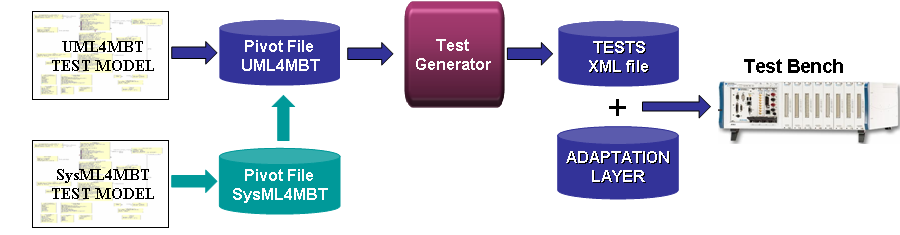
\includegraphics[width=\columnwidth]{./img/newToolChain.png}
        \caption{SysML4MBT toolchain.}
	\label{newToolChain}
\vspace*{-.35cm}
\end{figure}

The implementation of the \texttt{ComCover} approach is then performed
during the translation of the SysML4MBT model into the corresponding
UML4MBT model, as suggested in other Model-Based approaches such
as~\cite{weiss10}. More precisely, it consists to specialize the
translation rules of SysML4MBT into UML4MBT model such that applying
$All~transitions$ and D/CC strategies on UML4MBT resulting model
implies the coverage of the initial SysML4MBT model by $All~DU_{sig}$
and D/CC criteria. The next sections give details about
this implemented approach. 

\subsection{Model Transformation}
\vspace*{-.15cm}
SysML being a profile of UML, the majority of the rewriting rules to translate SysML4MBT
into UML4MBT models can be automatically performed by deleting the stereotype
layer of SysML (blocks become classes, block properties become class
attributes, block operations become class operation\ldots). For
specific SysML entities, the following dedicated translation rules are defined:

\begin{itemize}
  \vspace*{-0.25cm}
\item Each SysML4MBT signal is translated into a dedicated UML4MBT
    class. 
  \item Each receive port is translated into a link between the class
    representing the block hosting the port and each class
    representing each signal that can be received on this port. 
  \item The OCL operator circumflex is translated into an OCL
    expression that manipulates the link resulting from the
    translation of the receive ports
  \item Historic states are rewriting using a class attribute that
    simulates a memory state and related OCL constraints are added on
    transitions. 
  \item parallel structures (fork/join, parallel states and multiple
    Statemachines) are translated into sequential structures by
    applying a synchronized product. 
\end{itemize} 
The SysML4MBT model is thus automatically translated into an
equivalent UML4MBT model that can be used as input of the existing
test generation tool. The rules to translate SysML4MBT models into an equivalent UML4MBT models
are detailed and formalized in~\cite{UMLFM10}. 

\subsection{ComCover Implementation}
\vspace*{-.15cm}
To apply the \texttt{ComCover} strategy, specific transitions
have to be introduced during the translation from
SysML4MBT into UML4MBT model. These artificial behaviours concern each
signal send/receive couple, which defines the goal of the $All~DU_{sig}$
coverage criterion: each pair signal send/receive of the SysML4MBT
model is thus represented by one specific transition behaviour in the resulting
UML4MBT model. Since UML4MBT applies a selection strategy
based on the criteria $All$ $transitions$ and D/CC, we can ensure that
each pair signal send/receive is covered by the generated test cases. 
The implementation of this dedicated translation requires three steps. 
Firstly, at each generated UML4MBT class that denotes a SysML signal, 
an attribute is added. This attribute is an integer initialized to 0. 
Secondly, OCL expression are added to all behaviours sending a signal 
to update this attribute with a specific number: in this way, from
each receive behaviour, it is possible to know from which send behaviour 
the pending signal has been sent. Finally, a nested OCL conditional expression (each condition tests a particular value of the attribute) is added to each transition triggered by a signal receive. It artificially creates behaviours that are covered by the D/CC strategy. Covering these behaviours thus allows to ensure the $All~DU_{sig}$ coverage of the SysML4MBT model.  

\vspace*{-.25cm}
\subsection{Case Study Results}
\label{result}
\vspace*{-.15cm}

The \texttt{ComCover} selection strategy has been evaluated with four case 
studies:
 \vspace*{-.05cm}
\begin{itemize}
  \item $Lightings$ deals with the front lightings system of a
    car. This system allows to independently light on and light off
    headlights and highlights of the car using a control lever. The
    SysML4MBT model only contains simple one-to-one
    communications: the test cases generated using
    \texttt{ComCover} implementation are thus equivalent to those obtained
    by applying $All~transitions$ strategy. 
   \item $Lightings$ $Extended$ also concerns the study of a front
    lighting system of a car, but it considers the ignition subsystem
    and the control stick is replaced by a tactile panel. Thus,
    communications are more complex than $Lightings$ case study. The
    SysML4MBT model looks like smaller but contains, in fact, more
    functionalities. For instance, in this case study, an historic
    state adds complexity in the model, and the model manages much more
    signals. That is why the use of \texttt{ComCover} becomes relevant
    and more tests are generated and improves the coverage of the
    SysML4MBT test model.
   \item $Wiper$ specifies a wiper system of a car. Modeled
    functionalities are speed of drying up (low, high and
    intermittently) and windows cleaning with drying up. A lot of mechatronic parts being considered and communications being complex, a lot of relevant test cases are generated by the \texttt{ComCover} algorithm. 
    \item $Steering$ aims to examine behaviours of the steering column
    of a car, by observing reactions of the system contingent on road
    plots. In the SysML4MBT model, road characteristics are
    represented using blocks. Those blocks are linked to the steering
    column that defines the SUT. Test cases generated by
    \texttt{ComCover} are more relevant regarding mechatronic
    validation purpose, i.e. interactions between components and its
    environment.
\end{itemize}

Table~\ref{casestudies} summarizes the global metrics of the
experimentation results. From the second to the sixth line, the amount
of the different entities specified in the SysML4MBT test model is
given: Blocks, Connectors/Sending signal/Receive signal (c/s/r),
parallel Statemachines (SM), States, Transitions. $States$ 
(resp. $Transitions$) line details the number of states
(resp. transitions) of each Statemachine of the model. The lines
$All~transitions$ contain the number of tests generated using this
strategy, while \texttt{ComCover} line introduces the number of new
test cases produced by this coverage criterion. Finally, the line
$Total$ indicates how many test cases are generated by applying
both strategies. 

\begin{table}[!h]
\centering
\vspace*{-.4cm}
\caption{Case study results.}
\footnotesize{
	\begin{tabular}{|c|c|c|c|c|c|c|}
    	\hline
    	& & Emergency & Lightings & Lightings & Wiper & Steering \\
    	& & Stop & & Extended & &
    	\\ \hline
    	\multirow{7}{*}{\begin{turn}{90}{\scriptsize SysML4MBT \newline
    	model}\end{turn}}
		& Blocks & 4 & 6 & 4 & 15 & 9 \\ \cline{2-7}
    	& c/s/r & 1/2/2 & 4/8/4 & 8/14/10 & 26/58/65 & 10/25/20
    	\\ \cline{2-7}
    	& SM & 3 & 5 & 3 & 12 & 6
    	\\ \cline{2-7}
    	& States & (2,2,2) & (2,2,2,2,4) & (2,5,5) & (1,1,1,1,1,2, & (2,4,3,6,3,4) 
    	\\
    	& & & & & 17,10,2,2,2,2) &
    	\\ \cline{2-7}
    	& Transitions & (3,3,3) & (3,3,3,3,9) & (2,8,8) &
    	(2,3,2,4,1,3, & (3,8,4,5,9,8)
    	\\
    	& & & & & 52,16,2,2,2,2)&
    	\\ \hline
    	\multicolumn{2}{|l|}{$All~transitions$} &
    	4 & 8 & 17 & 85 & 35
    	\\ \hline
    	\multicolumn{2}{|l|}{ComCover (new tests)} &
    	1 & 0 & 8 & 19 & 26
    	\\ \hline
    	\multicolumn{2}{|l|}{Total} &
    	5 & 8 & 25 & 104 & 61 
    	\\ \hline
	
        \end{tabular}
	\label{casestudies}
}
\vspace*{-.4cm}
\end{table}

These case studies, presenting a growing complexity in terms of
model expressiveness and behavioral aspects, show that
\texttt{ComCover} can be successfully applied to embedded system domain. In the one hand, it ensures a
better coverage of communication issues specified in the test model,
as shown previously with the Emergency Stop case study. In the other hand, the number of new generated tests 
is manageable. In~\cite{JLAThesis2012}, we prove that, given $c$, $s$
and $r$ being respectively the number of Connectors, Sending signal
and Receive signal of a SysML4MBT specification, the maximum
number of new tests generated by \texttt{ComCover} is theoretically
equal to $(s-c+1)*(r-c+1)+(2c-r-s+1)$. But in practice, this maximum,
which defines the worst case (all the signals can be sent to and
received from all the connectors) is never reached. 

While $Lightings$, $Lightings Extended$ and $Wiper$ case studies have
been realized in an experimental way (the generated test cases have
been executed and studied using only a simulated version of the concrete
mechatronic system), $Steering$ case study gave rise to a complete
use of the toolchain (from the SysML4MBT test model to the execution of 
the generated test cases on a physical test bench. More concretely, 
the generated test cases have been
executed to validate a concrete physical Steering Column against a
Matlab/Simulink simulation model.
The Matlab/Simulink simulation model has been used as reference to
calculate the expected value on the concrete system. In this way, the
generated test cases have been executed on the physical test bench and
values calculated by the simulator were compared with the values
observed on the Test Bench. 

This realistic experimentation enables the detection of some errors
both in the simulation model and in the concrete system configuration. More
details about this end-to-end toolchain and the experimentation results
on this case study have been respectively published in~\cite{LPG11} and~\cite{ABLLP12}. A short videotape, exemplifying it, is also 
available\footnote{VETESS project web site - \url{http://lifc.univ-fcomte.fr/vetess/}}. This
experimentation, as well as the other case studies in a less realistic
manner, enabled to validate our approach. They show its relevance for embedded 
mechatronic systems, which strongly
rely on subsystem communication, by focusing the test objectives on
signal exchanges.

\vspace*{-.3cm}
\section{Conclusion and Future Work}
\label{conclusion}
\vspace*{-.3cm}
This paper proposes original coverage criteria ($All~DU_{sig}$
and $All~DU_{sig}-paths$) to increase the model coverage, within MBT
approach from \textit{Systems Modeling Language}, to validate
mechatronic systems. These criteria are based on a Def-Use approach
focused on the communication features of the SysML test model. A
dedicated test selection strategy, called \texttt{ComCover}, has been
defined and implemented to automatically generate test cases covering
the $All~DU_{sig}$ criterion. This strategy aims to improve an
existing MBT process by considering communicating embedded systems
modeled using SysML. However, this result is
not restricted to this process and can be applied in all approaches
that consider systems defined by material and logical subparts that
communicates to each other. Finally, this automated toolchain has been
experimented with industrial case studies, which allow to highlight the 
relevance of the \texttt{ComCover} strategy to
generate test cases for  communicating system. 
We are now investigating the use of real-time constraints to complete
the SysML4MBT test model and improve the
relevance of test cases for real-time systems.
This model feature, major aspect of embedded system domain, will be
addressed using UML MARTE profile.  
\vspace*{-.3cm}
\bibliographystyle{splncs}
\bibliography{63_biblio} 
\end{document}

